\documentclass[a4paper,14pt]{extreport}

\newcommand{\globalEncoding}{utf8}		% кодировка	
\newcommand{\globalStylesDir}{"E:/Documents/Git/graduateWorkStyle"}	% месторасположение стилей
\newcommand{\globalSourceDir}{src}	% месторасположение кодов
\newcommand{\globalPictureDir}{pic}	% месторасположение изображений

% подключаем набор стилей
\usepackage{\globalStylesDir/graduateWorkMain}
\renewcommand{\itshape}{}
\usepackage{lscape}
\selectlanguage{russian}
\begin{document}
	% Tитульная страница
	\title{Разработка ПО для автоматизации конфигурирования сетевого оборудования CISCO}
	\subtitle{Отчет по преддипломной практике}
	\teachers{2}{Трофимов С.П.}
	\students{1}{Черетаев И.В.}
	\specialty{Информатика и вычислительная техника}
	\group{РИ-420207}
	\city{Екатеринбург}		
	\maketitle
	\setcounter{page}{2} % начать нумерацию страниц с №2
	
	% Оглавление
	\tableofcontents
	
	\chapter*{Введение}
	\addcontentsline{toc}{chapter}{ВВЕДЕНИЕ}
	
	Во второй половине прошлого века в связи с «рождением» первых
	вычислительных сетей произошла очередная научно-техническая революция. Появилась возможность начать использование рассредоточенной
	обработки данных, обширно использовать для автоматизации различных
	видов деятельности новые технологии. В наши дни даже маленький ребенок имеет представление о компьютерных сетях, и, в то же время,
	наладка сетевого оборудования является довольно кропотливым делом,
	которое не терпит небрежного отношения.
	
	В наше время происходит активное применение сетевых решений во многих сферах деятельности. В условиях производства, на различных предприятиях,
	в офисах компаний, различных фирмах и учреждениях отдельно стоящий, не подключенный к сети компьютер является большой редкостью. Можно смело заявлять, что через какое-то время
	большая часть компьютеров будет включено в те или иные сети. Если же
	подобной сети в учреждении нет или она плохо развита, нет сомнений,
	что ей придется развиваться.
	
	Основным моментом в данном вопросе является технический прогресс, постоянно обеспечивающий нас новыми возможностями, но накладывающим на технических специалистов высокие требования, в частности – необходимость повышенной адаптивности. Несмотря на это,
	для специалистов наладка сетевого оборудования являет собой одно из
	основных направлений, где качество безоговорочно удерживает пальму
	первенства по важности.
	
	Одним из представителей компаний-производителей сетевого оборудования является Cisco Systems. Cisco Systems — компания-производитель
	сетевого оборудования, основанная в 1984. Сначала компания производила маршрутизаторы, но затем значительно расширила ассортимент своей продукции. В настоящее время она производит коммутаторы, маршрутизаторы,
	IP-телефоны, программное обеспечение для своего оборудования.
	
	Огромное сообщество сетевых администраторов, IT-специалистов, студентов не всегда хочет привлекать квалифицированных специалистов
	Cisco для того, чтобы быстро запустить какой-либо проект на оборудовании Cisco. Они обычно нуждается в простом, работающем решении,
	позволяющее им не посвящать остаток жизни изучению всех тонкостей сетевых технологий, маршрутизации, информационной безопасности, беспроводной связи и т.д.
	
	Соответственно, необходимо решение, которое быстро и легко поможет настроить оборудование Cisco и решить данные проблемы.
	
	\chapter{Обзор существующих решений}
	
	Рассмотрим несколько приложений, решающих задачу автоматизации
	конфигурирования сетевого оборудования Cisco.
	
	Сначала несколько слов по терминологии.
	
	Симуляторы — реализуют статичное множество команд, но, только
	пользователь выходит за рамки возможного, выдают сообщение об ошибке. Классическим примером является Cisco Packet Tracer.
	
	Эмуляторы — дают возможность выполнять команды образов настоящих устройств, порой без заметных урезаний функциональности. Эмулятором, к примеру, является GNS3/Dynamips.
	
	\section{Cisco Packet Tracer}
	
	
	Начнем обзор с Packet Tracet (см рис. \ref{fig:packet_tracer}) – официального выпускаемого Cisco
	программного обеспечения. Данный продукт доступен в версиях как для
	Windows, так и для Linux, бесплатно для учащихся Сетевой Академии
	Cisco.
	
	Вся настройка осуществляется при помощи логической диаграммы сети, для моделирования доступен большой набор оборудования, выпускаемого Cisco и не только (маршрутизаторвы, коммутаторы, персональные компьютеры и многое другое).
	
	Достоинства Packet Tracet — дружественность и логичность интерфейса. Также, в нем удобно проверять функционирование различных сетевых сервисов, например DHCP или DNS. И одно из самых интересных преимуществ — это
	возможность перейти в режим симуляции и увидеть все действия с
	пакетами с использованием замедления времени.
	
	Однако, стоит заметить, что реализованная функциональность устройств
	ограничена и не предоставляет всех возможностей реального оборудования. Большим минусом является тот факт, что некоторые команды не
	поддерживает. Почти всё, что не входит в программу изучения CCNA, на нем собрать
	не получится.
	
	
	\begin{figure}[h]
		\centering
		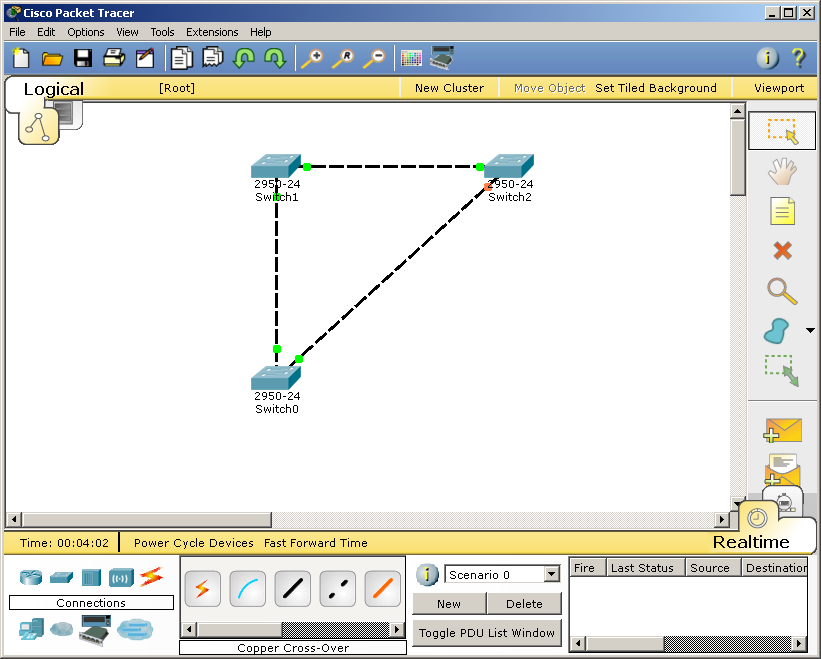
\includegraphics[width=0.9\linewidth]{pic/packet_tracer}
		\caption{Cisco Packet Tracer}
		\label{fig:packet_tracer}
	\end{figure}
	
	\section{GNS3}
	
	
	Следующий продукт в обзоре — GNS3, представляющий собой графический интерфейс, написанный на Qt, для эмулятора dynamips (см. рис. \ref{fig:gns3}).
	Является свободно распространяемым проектом и доступен под следующими операционными системами: Linux, Windows и Mac OS X.
	
	В то же время, большинство его функций, призванных улучшить производитель-
	ность, работают только под Linux, 64 битная версия так же только для Linux.
	
	Это эмулятор, который работает с оригинальными прошивками IOS.
	Это означает, что для использования GNS3, вам необходимо иметь в наличии реальные образы.
	
	\begin{figure}[h]
		\centering
		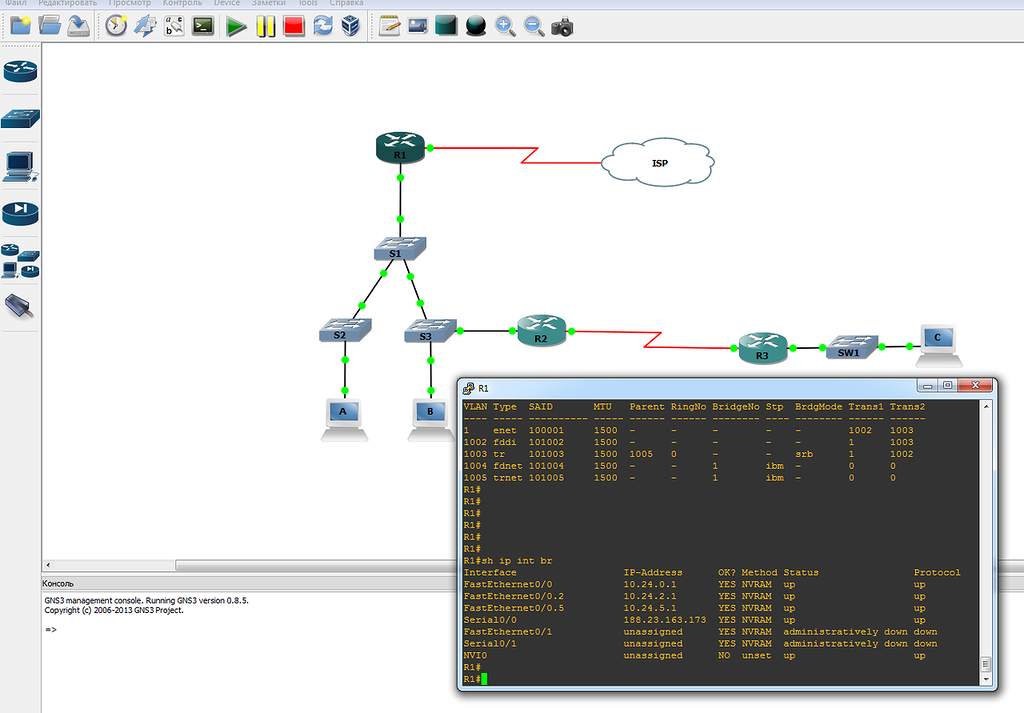
\includegraphics[width=0.9\linewidth]{pic/gns3}
		\caption{GNS3}
		\label{fig:gns3}
	\end{figure}
	
	
	
	Так же имеется несколько других недостатков:
	\begin{itemize}
		\item ограниченное число платформ;
		\item невозможность полноценно использовать коммутаторы Catalyst;
		\item уменьшение производительности при использовании огромного количества устройств.
	\end{itemize}
		
	\section{Boson NetSim}
	
	Доступен в версии только для Windows, цена колеблется от 179$ за CCNA
	и до 349$ за CCNP.
	
	Выступает в роли набора лабораторных работ, объединенных по темам экзамена. Интерфейс разделен на нескольких разделов: постановка задачи, карта сети, в
	левой части находится список доступных лабораторных работ (см. рис. \ref{fig:netsim}).
	
	По завершении работы, можно получить результат и узнать все ли было
	сделано.
	
	Присутствует возможность создания собственных топологий, с некоторыми
	ограничениями.
	
	
	\begin{figure}
		\centering
		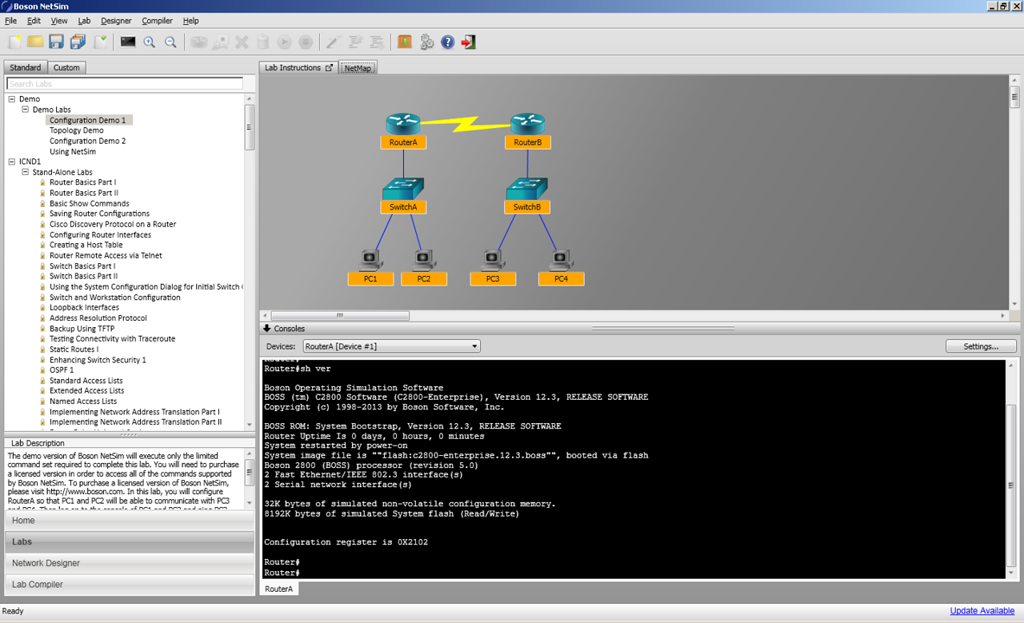
\includegraphics[width=0.9\linewidth]{pic/netsim}
		\caption{Boson NetSim}
		\label{fig:netsim}
	\end{figure}
	
	Ключевые возможности Boson NetSim:
	
	\begin{itemize}
		\item поддержка  42 маршрутизаторов, 6 коммутаторов;
		\item симуляция сетевого трафика при помощи технологии виртуальных
		пакетов;
		\item два режима просмотра: telnet или подключение по консоли;
		\item возможность создания собственных лабораторий.
	\end{itemize}
	
	

	
	\section{Cisco IOU}
	
	Последний в этом списке это  Cisco IOU (Cisco IOS on UNIX) —
	проприетарное ПО, которое официально не распространяется (см. рис. \ref*{fig:ciscoIOU}).
	
	\begin{figure}[h!]
		\centering
		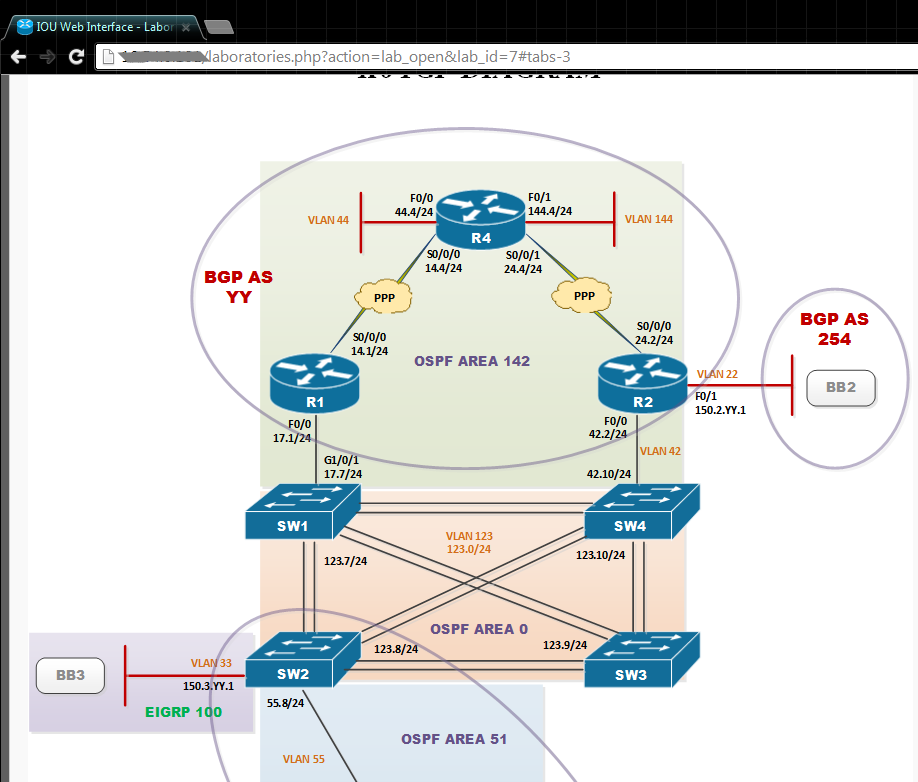
\includegraphics[width=0.7\linewidth]{pic/ciscoIOU}
		\caption{Cisco IOU}
		\label{fig:ciscoIOU}
	\end{figure}
	
	Существует мнение, что у Cisco есть возможность отследить и идентифицировать того, кто использует IOU.
	Известный факт состоит в том, что центр технической поддержки Cisco использует именно данных продукт.
	
	Сначала  был доступен только под Solaris, но затем был портирован и
	на Linux. В комплекте идут две основные части --- l2iou и l3iou. Первая часть эмулирует канальный уровень и коммутаторы, вторая же — сетевой уровень и маршрутизаторы.
	
	Настройка проводится путем редактирования конфигурационных файлов, недавно для него стал доступен также графический интерфейс.
	
	Интерфейс довольно интуитивен, и позволяет выполнять почти все действия.
	
	Включение на моделирование топологии, указанной на рис. \ref{fig:topologyCCIE}, приводит примерно к 20\%
	загрузке процессора.
	
	\begin{figure}[h!]
		\centering
		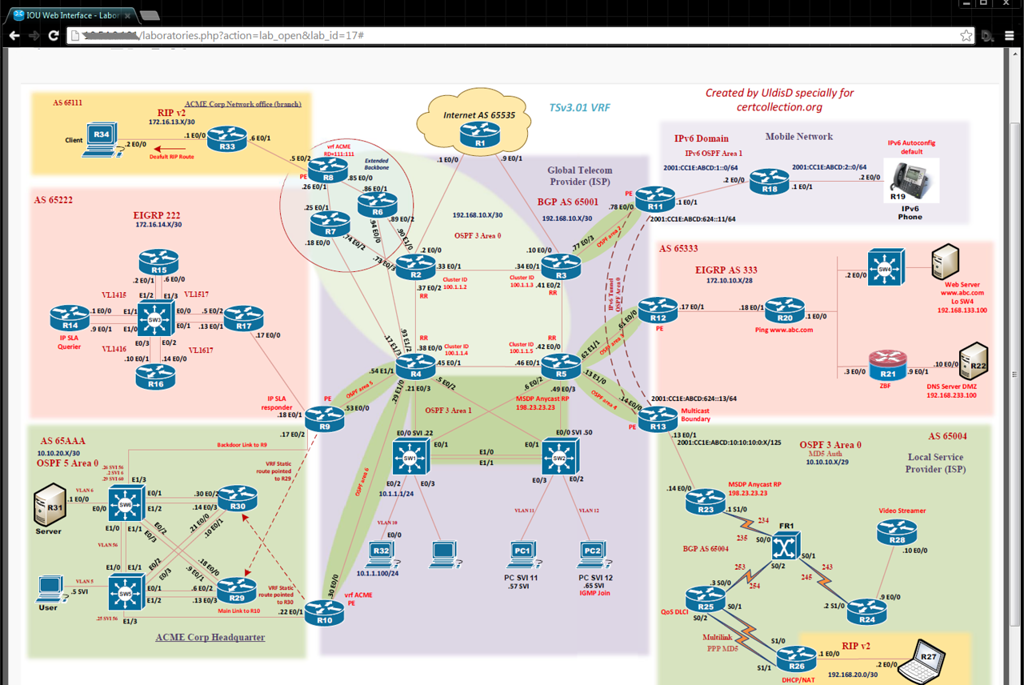
\includegraphics[width=0.7\linewidth]{pic/topologyCCIE}
		\caption{Пример топологии}
		\label{fig:topologyCCIE}
	\end{figure}
	
	Надо сказать, данная топология предназначена для подготовки к сдаче экзамена на Cisco Certified Internetwork Expert.
	
	Возможности IOU на самом деле очень широкие. В тоже время, некоторые проблемы на канальном уровне все же имеются. Для некоторых устройств, например, отсутствует возможность жестко выставить дуплексный режим, но это всё мелочи.
	
%	\begin{longtable}{|p{8,5cm}|p{4cm}|p{4cm}|} % описываем 3 столбца таблицы с выравниванием по ширине и указанной ширины
%		% Вертикальная черта означает, что между полями должна быть вертикальная черта - разделитель
%		% Заголовок таблицы на первой странице:
%		\caption{Исходные данные по работе <<Проект сети широкополосного доступа на базе FTTH>>\label{tab:econ_effect}}\\
%		\hline % Вставляем горизонтальную линию
%		Наименование показателей & Единица измерения & Значение показателей \\
%		\hline
%		\endfirsthead % Всё, что расположено выше считается заголовком таблицы и отображается на первой странице
%		% Для второй и последующих страниц подменяем наименование таблицы в соответствии с требованиями:
%		\caption*{Продолжение таблицы \ref{tab:econ_effect}}\\
%		\hline
%		\centering 1 & \centering 2 & \centering 3 \\
%		\endhead % Всё что выше будет вставляться как заголовок на 2 и последующих страницах
%		\hline
%		1 Объем услуг & & \\ % Содержимое ячеек разделяется знаком &, завершение строки таблицы \\
%		\hline
%		Сеть доступа: & абонентов & 384 \\
%		\hline
%		В том числе: & & \\
%		\hline
%		юридические лица & абонентов & 38 \\
%		\hline
%		физические лица & абонентов & 346 \\
%		\hline
%		Доля физических лиц & & \\
%		\hline
%		Пакет №1 (высокоскоростной Интернет) & \% & 65 \\
%		\hline
%		Пакет №2 (Интернет + IP TV) & \% & 22 \\
%		\hline
%		Пакет №3 (Интернет + IP TV + VoD) & \% & 13 \\
%		\hline
%		Доля юридических лиц & & \\
%		\hline
%		Пакет №1 (Интернет) & \% & 69 \\
%		\hline
%		Пакет №2 (IP VPN) & \% & 31 \\
%		\hline
%	\end{longtable}
	\begin{landscape}
		\begin{longtable}{|p{3.5cm}|p{5cm}|p{5cm}|p{5cm}|p{5cm}|} 
		% Вертикальная черта означает, что между полями должна быть вертикальная черта - разделитель
		% Заголовок таблицы на первой странице:
		\caption{Сравнение существующих решений\label{tab:econ_effect}}\\
		\hline % Вставляем горизонтальную линию
		{\centering Наименование показателей} & \centering Cisco Packet Tracer & \centering GNS3  & \centering Boson NetSim & Cisco IOU \\
		\hline
		\endfirsthead % Всё, что расположено выше считается заголовком таблицы и отображается на первой странице
		% Для второй и последующих страниц подменяем наименование таблицы в соответствии с требованиями:
		\caption*{Продолжение таблицы \ref{tab:econ_effect}}\\
		\hline
		\centering 1 & \centering 2 & \centering 3 \\
		\endhead % Всё что выше будет вставляться как заголовок на 2 и последующих страницах
		\hline
		
		Тип решения & симулятор & эмулятор & симулятор & симулятор \\
		\hline
		Ценовая политика & доступен студентам сетевой академии Cisco & бесплатен & от 179\$ за CCNA и до 349\$ за CCNP & проприетарен \\
		\hline
		Версии ОС & Windows, Linux & Linux, Windows и Mac OS X & Windows & Solaris, Linux \\
		
		
		
		\hline
	\end{longtable}
	
	Общим недостатком представленных программных продуктов можно назвать излишнюю комплексность решения, вызванную попытками смоделировать полное поведение сетевых технологий, что, в свою очередь, вызывает дальнейшие сложности при освоении.
	\end{landscape}
	
	\chapter{Выбор инструментальной системы разработки ПО}
	
	В ходе прохождения преддипломной практики были рассмотрены несколько инструментальных сред разработки на C/C++. В связи с тем проект некоммерческий, в списке присутствуют только бесплатные программные продукты.
	
	\section{Code::Blocks}
	
	Разработчики Code::Blocks выбрали путь открытой архитектуры, позволив сторонним программистам повышать
	эффективность программы за счет собственных разработок (плагинов). Об одном из плагинов
	нужно сказать отдельно - wxSmith, который, по сути, является  wxWidgets
	RAD инструментом, то есть позволяет создавать оконные формы и прочие графические объекты, используя библиотеку wxWidgets (библиотека
	wxWidgets устанавливается отдельно). 
	
	Плюсы Code::Blocks:
	
	 \begin{itemize}
		 \item подсветка кода;
		 \item автозавершение кода;
		 \item просмотрщик классов;
		 \item быстрая система сборки (не требуются make-файлы);
		 \item поддержка параллельных сборок.
	 \end{itemize}
	 
	\section{Microsoft Visual Studio Express}
	
	
	Эта версия Visual Studio представляет собой набор урезанных средств
	разработки для языков Visual Basic, C\# и C++, и обозначается Microsoft как инструментальная среда разработки начального
	уровня для тех лиц, кто не занимается профессионально программированием
	(школьников, студентов, любителей и т.д.).
	
	Графический интерфейс и возможность создать оконные приложения присутствует, но возможность воспользоваться наработками компании в области оптимизации и рефакторинга кода почти отсутствует.
	
	\section{Qt Creator}
	
	Qt Creator является средой разработки для кроссплатформенного фреймворка Qt. Вследствие этого, нужно указать на следующие его возможности:
	\begin{itemize}
		\item интеграция дизайнера форм Qt и справочной системы Qt
		\item расширяемость (посредством плагинов)
		\item поддержка дебагеров GDB (графический фронтенд) и CDB
		\item подсветка кода с поддержкой нескольких языков и разметок
	\end{itemize}
	
	
	
	\begin{longtable}{|p{3.5cm}|p{3.5cm}|p{4cm}|p{3.5cm}|} 
		% Вертикальная черта означает, что между полями должна быть вертикальная черта - разделитель
		% Заголовок таблицы на первой странице:
		\caption{Сравнение IDE\label{tab:ide_effect}}\\
		\hline % Вставляем горизонтальную линию
	Наименование показателей &  \centering Code::Blocks & \centering Microsoft Visual Studio Express & \centering Qt Creator\\
		\hline
		\endfirsthead % Всё, что расположено выше считается заголовком таблицы и отображается на первой странице
		% Для второй и последующих страниц подменяем наименование таблицы в соответствии с требованиями:
		\caption*{Продолжение таблицы \ref{tab:ide_effect}}\\
		\hline
		\multicolumn{1}{|c|}{1} & \multicolumn{1}{|c|}{2 } & \multicolumn{1}{|c|}{3} & \multicolumn{1}{|c|}{4}\\
		\endhead % Всё что выше будет вставляться как заголовок на 2 и последующих страницах
		\hline
		
		Лицензия & \multicolumn{1}{c|}{GPL} & \multicolumn{1}{c|}{Freeware} & \multicolumn{1}{c|}{GPL} \\
		\hline
		Кроссплат\-форменность & \multicolumn{1}{c|}{Да} & \multicolumn{1}{c|}{Нет} & \multicolumn{1}{|c|}{Да}  \\
		\hline
		Разработка GUI & \multicolumn{1}{c|}{Да\footnote{С использованием плагина wxSmith}} & \multicolumn{1}{c|}{Да} & \multicolumn{1}{|c|}{Да} \\
		
		\hline
	\end{longtable}
	
	
	Исходя из приведенных выше сведений, было принято решение, что приложение будет написано в среде Qt Creator с использованием кроссплатформенного фреймворка Qt на языке C++. Это позволит сократить время на разработку, избежать написания большого количества кода, посредством использования готовых библиотек. Использование библиотеки Qt также поможет создать удобный интерфейс, отличный от стандартного.
	
	\chapter{Техническое задание}
	
	\section{Общие сведения}
	
	\subsection{Полное наименование системы и ее условное обозначение}
	
	Программное обеспечение для автоматизации конфигурирования сетевого оборудования Cisco. Условное обозначение – АКСО\cite{gost-19.201-78}.
	
	\subsection{Краткая характеристика области применения}
	
	АКСО предназначено для автоматизации конфигурирования сетевого оборудования Cisco путем предоставления пользователю графического интерфейса с последующим получением набора команд, необходимых для внедрения изменений внесенных пользователем.
	
	\subsection{Перечень документов, на основании которых создается система}
	
	\begin{enumerate}
		\item Приказ ректора УрФУ № \_\_\_\_\_\_ от "\_\_\_"\_\_\_\_\_\_\_\_\_\_ \_\_\_\_\_г.
	\end{enumerate}
		
	\subsection{Перечень документов, на основании которых устанавливается порядок оформления и предъявления результатов работ}
	
	\begin{enumerate}
		\item  Методические указания по выполнению выпускной квалификационной работы бакалавра техники и технологий по направлению "Информатика и вычислительная техника" / сост. А.Б.Николаев. – Москва: МАДИ, 2010. – 17 с.
		\item Соколов С.С. Рекомендации по оформлению курсовых, выпускных и дипломных проектов (работ). Электронные методические указания - Екатеринбург: Изд. УрФУ, 2010. - 38 с.
	\end{enumerate}
	
	
	\section{Назначение разработки}
	
	\subsection{Функциональное назначение}
	
	Функциональным назначением АКСО является предоставлению пользователю удобных инструментов для облегчения конфигурирования сетевого оборудования от компании Cisco Systems, таких как маршрутизаторы и/или коммутаторы.
	
	\subsection{Эксплуатационное назначение}
	
	АКСО предназначено для автоматизации процесса конфигурирования сетевого оборудования с целью получения исходного текста конфигурации либо автоматического применения внесенных с помощью АКСО изменений на сетевом оборудовании.
	
	\section{Требования к программному средству}
	
	\subsection{Требования к функциям, выполняемым системой }
	
	\begin{enumerate}
%		\item Разработать структуру классов, хранящую информацию о сетевых устройствах.
		
		\item Наличие основных моделей маршрутизаторов и коммутаторов.
		
		\item Наличие редактора, позволяющего добавлять новые модели (в том числе, на основе уже существующих моделей), изменять и удалять существующие. Редактор должен обеспечивать возможность поиска в списке имеющихся моделей. Так же при помощи данного редактора должны производиться операции визуального изменения конфигурации для выбранного модели сетевого оборудования.
		
		\item Наличие возможности экпорта/импорта выбранной конфигурации в виде XML-файла, содержащего все необходимые сведения.
		
		\item Наличие возможности сохранения выбранной конфигурации в виде текстового файла, содержащего команды конфигурирования
		
		\item Наличие справочную подсистему. Справка должна содержать краткую информацию о системе и ее возможностях, описание действий пользователя и получаемых результатов при работе с программным обеспечением.
	\end{enumerate}
	
	\subsection{Требования к надежности функционирования и безопасности}
	
	Надёжность системы должна обеспечивать работоспособность в течение всего срока эксплуатации при бесперебойном питании ЭВМ. Программное обеспечение не должно содержать явных логических ошибок и функционировать без сбоев.	
	
	\subsection{Требования к информационной и программной совместимости}
	
	АКСО должна иметь возможность функционировать под управлением различных операционных систем (Windows, Linux и т.д.).
	
	\subsection{Требования к исходным кодам и языкам программирования}
	
	Исходные коды программного средства должны быть реализованы на языке C++. В качестве интегрированной среды разработки программы должна быть использована среда Qt Creator.
	
	\subsection{Специальные требования}

	Программа должна обеспечивать взаимодействие с пользователем (оператором) посредством графического пользовательского интерфейса.
	
	\section{Стадии и этапы разработки}
	
	\subsection{Стадии разработки}
	
	Разработка должна быть произведена в три стадии\cite{iso-12207}:
	\begin{enumerate}
		\item Разработка технического задания;
		\item Рабочее проектирование;
		\item Внедрение;
	\end{enumerate}
	
	\subsection{Этапы разработки}
	На стадии рабочего проектирования должны быть выполнены перечисленные ниже этапы работ:
	\begin{enumerate}
		\item разработка АКСО; 
		\item разработка программной документации; 
		\item испытания АКСО.
	\end{enumerate}
	
	На стадии внедрения должен быть выполнен этап разработки - подготовка АКСО.
	
	\subsection{Содержание работ по этапам}
	
	На этапе разработки АКСО должна быть выполнена работа по программированию (кодированию) и отладке программного обеспечения (АКСО).
	
	На этапе разработки программной документации должна быть выполнена разработка программных документов в соответствии с требованием п. \ref{subsection:documentation} настоящего технического задания.
	
	На этапе испытаний АКСО должны быть выполнены перечисленные ниже виды работ:
	
	\begin{enumerate}
		\item проверка выполнения заданных функций АКСО;
		\item выявления и устранения недостатков в АКСО и программной документации; 
		\item корректировка АКСО и программной документации по результатам тестирований.
	\end{enumerate}
	
	На этапе подготовки АКСО должна быть выполнена работа по подготовке программного средства и программной документации для эксплуатации.
	
	\section{Порядок защиты и контроля}
	
	Защита осуществляется перед Государственной аттестационной комиссией (ГАК), утвержденной приказом ректора.
	
	\section{Требования к программной докуменации}
	\subsection{Предварительный состав программной документации}
	\label{subsection:documentation}
	Предварительный состав программной документации должен включать в себя\cite{gostr-9294}:
\begin{enumerate}
	\item техническое задание;
	\item текст программы;
	\item описание программы;
	\item пояснительную записку\cite{methodVKR,methodVKRUrFU};
	\item руководство пользователя.
\end{enumerate}
	
	
	

	
	\section{Источники разработки}
	\begin{enumerate}
%		\item ГОСТ 19.201-78. Техническое задание, требования к содержанию и оформлению. 
%		\item ГОСТ 19.102-77 ЕСПД. Стадии разработки. 
%		\item ГОСТ 19.104-78 ЕСПД. Основные надписи. 
%		\item ГОСТ 19.105-78 ЕСПД. Общие требования к программным документам. 
%		\item ГОСТ 19.106-78 ЕСПД. Требования к программным документам, выполненным печатным способом. 
%		\item ГОСТ 28195-89. Оценка качества программных средств. Общие положения.
%		\item ГОСТ 19.781-90. Обеспечение систем обработки информации программное. Термины и определения
%		\item  Методические указания по выполнению выпускной квалификационной работы бакалавра техники и технологий по направлению "Информатика и вычислительная техника" / сост. А.Б.Николаев. – Москва: МАДИ, 2010. – 17 с.
%		\item Методические указания к выполнению выпускных бакалаврских работ по направлению 552800 «Информатика и вычислительная техника» по специальности 230101 65 «Вычислительные машины, комплексы, системы, сети»/Под общей ред.В.А.Бархоткина. - Москва:МИЭТ, 2006. - 15с.
%		\item Соколов С.С. Рекомендации по оформлению курсовых, выпускных и дипломных проектов (работ). Электронные методические указания - Екатеринбург: Изд. УрФУ, 2010. - 38 с.


%		\item ГОСТ 19.102-77 ЕСПД. Стадии разработки.
%		\item ГОСТ 19.105-78 ЕСПД. Общие требования к программным доку-
%		ментам.
%		\item ГОСТ 19.106-78 ЕСПД. Требования к программным документам,
%		выполненным печатным способом.
		\item ГОСТ 19.201-78. Техническое задание, требования к содержанию и оформлению.
		\item ГОСТ Р ИСО/МЭК 9294-93 Информационная технология. Руководство по управлению документированием программного обеспечения.
		\item ISO/IEC 12207:2008 (ГОСТ Р) Системная и программная инженерия. Процессы жизненного цикла программных средств.
		\item ISO/IEC 9126:1991 (ГОСТ Р) Информационные технологии. Оценка программного продукта. Характеристики качества и порядок их применения.
	\end{enumerate}
	
	


	
	\chapter*{Заключение}
	\addcontentsline{toc}{chapter}{ЗАКЛЮЧЕНИЕ}
	
	Актуальность темы дипломной работы определяется быстрым ростом количества компаний, имеющих сложную информационную структуру. Наряду с этим возникает необходимость настройки огромного количества активного сетевого оборудования.	
	Все эти факторы приводят к тому, что администраторам информационной инфраструктуры компании приходится тратить много времени на порой рутинные работы.
	
	Цель дипломной работы состоит в разработке системы для автоматизированного создания конфигурационных файлов оборудования.
	
	Поставленная цель обусловила следующие задачи дипломной работы:
	
	\begin{itemize}
		\item определить сущности проектируемой системы и архитектуру их взаимодействия;
		\item реализовать систему в виде кроссплатформенного приложения с графическим интерфейсом;
		\item провести тестированием в лабораторной среде.
	\end{itemize}
	
	Объектом исследования выступает сетевое оборудование Cisco Systems.
	
	Предметом исследования в дипломной работе являются современные средства коммуникации и их интеграция в методы управления информационной инфраструктурой для повышения таких аспектов информационной безопасности предприятия, как целостность и доступность.
	
	Теоретическая значимость дипломного исследования состоит в развитии и совершенствовании методологии управления оборудованием информационной инфраструктуры предприятия.
	
	Практическая значимость работы определяется тем, что ее результаты позволяют повысить степень эффективности управления информационной инфраструктурой предприятия и снизить связанные с этим операционные расходы при использовании разработанной системы, направленной на повышение уровня таких аспектов администрирование, как быстрота и легкость обслуживания.
	
	Новизна дипломной работы заключается в разработке и реализации кроссплатформенной модели автоматизации конфигурирования оборудования.
	
	
	\appendix
	
	
	\titleformat{\chapter}[hang]
	{\filleft}
	{}{1pt}{\MakeUppercase}
%	
%
%	
%	\newappendix{Пример приложения}


	\renewcommand{\bibname}{Список использованных источников}
	\addcontentsline{toc}{chapter}{\bibname}
	\bibliographystyle{plain}
%	\bibliographystyle{gost780s} % ГОСТ 7.80
	\bibliography{bib/lit}	
\end{document}    